% !TEX root = ../paper.tex

\section{Numerical Experiments}\label{sec:exps_distr}

In this section, we demonstrate the relevance of our approach for joint clustering and DR,  over 8 labeled datasets detailed in \Cref{sec:exps_distr} including: 3 image datasets (COIL-20 \citep{nene1996columbia}, MNIST and fashion-MNIST \citep{xiao2017fashion}) and 5 genomic ones (PBMC \citep{wolf2018scanpy}, SNA 1 and 2 \citep{chen2019high} and ZEISEL 1 and 2 \citep{zeisel2015cell}). To this end, we examine how effectively DistR prototypes offer discriminative representations of input samples at various granularities, using an evaluation system described below.

\paragraph{Benchmarked methods.}
Let us recall that any DR method presented in \Cref{sec:background_dr} is fully characterized by a triplet $(L, \simiX, \simiZ)$ of loss and pairwise similarity functions.
Given such triplet, we compare our DistR model against sequential approaches of DR and clustering, namely \emph{DR then clustering} (DR$\to$C) and \emph{Clustering then DR} (C$\to$DR). These 2-step methods are representative of current practice in the field of joint clustering and DR \citep{baran2019metacell}. DR$\to$C representations are constructed by first running the DR method associated with $(L, \simiX, \simiZ)$ thus obtaining an intermediate representation $\widetilde{\mZ} \in \R^{N \times d}$. Then, spectral clustering \citep{von2007tutorial} on the similarity matrix $\simiZ(\widetilde{\mZ})$ is performed to compute a cluster assignment matrix $\widetilde{\mT} \in \R^{N \times n}$. The final reduced representation in $\R^{n \times d}$ is the average of each point per cluster, \ie the collection of the centroids, which is formally $\diag(\tilde{\vh})^{-1} \widetilde{\mT}^\top \widetilde{\mZ} \in \R^{n \times d}$ where $\tilde{\vh} = \widetilde{\mT}^\top \one_N$.
For C$\to$DR, a cluster assignment matrix $\widehat{\mT} \in \R^{N \times n}$ is first computed using spectral clustering on $\simiX(\mX)$.
Then, the cluster centroid $\diag(\hat{\vh})^{-1} \widehat{\mT}^\top \mX$, where $\hat{\vh} = \widehat{\mT}^\top \bm{1}_N$, is passed as input to the DR method associated with $(L, \simiX, \simiZ)$. Therefore the three methods produce a sample-to-prototype association matrix (formally described in \Cref{sec:implementation_details}) further used to evaluate performance.

For the choices of $(L, \simiX, \simiZ)$, we experiment with both spectral and neighbor embedding methods (NE). For the former, we consider the usual PCA setting with $d = 10$. Regarding NE, we rely on the \emph{Symmetric Entropic Affinity} (SEA) from \citep{van2023snekhorn} for $\simiX$ and the scalar-normalized student similarity for $\simiZ$ \citep{van2008visualizing}, setting the dimension $d=2$ as it coincides with real-life visualization purposes while outperforming PCA-based approaches. The SEA is robust to varying noise levels and depends on a certain perplexity parameter. We report validated hyperparemeters (\emph{e.g perplexity, number of prototypes $n$}) with additional implementation details in \Cref{sec:implementation_details}, and provide our code with the submission. 

\paragraph{Evaluation metrics.}
We consider several evaluation metrics to quantify whether the output prototypes provide a meaningful summarized representation of the input datasets. As often done in the literature, we focus on supervised evaluations while assessing two main properties.
Firstly, we wonder whether the prototypes are \emph{individually} discriminating
input samples $\{\vx_i\}$ w.r.t their class labels $\{y_i\}$ via their
associated prototype. We thus
compute the homogeneity score \citep{rosenberg2007v} that quantifies to which
extent each prototype $\vz_k$ is associated with points in the same class. 
Secondly, we aim to evaluate whether the embedding space is both \emph{globally discriminant}, \ie that prototypes organize themselves to form clusters that match the classes, measured by two metrics. \emph{i)} 
We associate with each prototype $\vz_k$ a label using majority voting from the associated samples.

Then we make use of the
popular silhouette score \citep{rousseeuw1987silhouettes} to evaluate whether
prototypes' positions are correctly aligned with these labels. \emph{ii)} As
commonly done to assess DR representations \citep{huang2022towards}, we also consider
the downstream task of clustering the prototypes using the k-means algorithm.
We then assign to each $\{\vx_i\}$ %input data point
the cluster of its associated prototype, acting as a predicted label, and compute the Normalized Mutual Information (NMI) \citep{kvaalseth2017normalized} between these labels and $\{y_i\}$.  %the ground truth labels.
% More details about evaluation metrics can be found in \Cref{sec:appendix_exps}.

\paragraph{Details on the scores.} The homogeneity and NMI scores are taken from \texttt{Torchmetrics} \citep{detlefsen2022torchmetrics}. The other scores used in the experiments are computed as follows.

\textit{i) Silhouette}: The first step is to associate a label with each prototype $\vz_k$ defined by the $y$ maximizing $\sum_{i \in \integ{N}} T_{ik} \bm{1}_{y_i = y}$ where $y_i$ is the class label of the input data point $\vx_i$. Then, to incorporate the relative importance $w_i = \left[\vh_Z\right]_i$ of each prototype $\vz_i$, we define the \emph{weighted} mean intra-cluster and nearest-cluster distances that read 
	\begin{equation}
		a_i (\mZ, \mY, \vw)= \frac{\sum_{j\in \integ{N} \delta_{y_i =y_j} w_j d(\vz_j, \vz_j)}}{\sum_{j \in \integ{N} \delta_{y_i = y_j} w_j }} \quad \text{and} \quad b_i (\mZ, \mY, \vw)= \frac{\sum_{j \in \integ{N}} \delta_{y_j = k} w_j d(\vz_j, \vz_i)}{ \sum_{j \in \integ{N}} \delta_{y_j = k}w_j }
	\end{equation}
	such that the silhouette coefficient is $s_i(\mZ, \mY, \vw) = \frac{b_i - a_i}{\max(b_i, a_i)}$ and the final silhouette score reads as
	\begin{equation}
		S(\mZ, \mY, \vw) = \sum_{i \in \integ{N}} w_i s_i(\mZ, \mY, \vw) \:.
	\end{equation}

\textit{ii) k-means}: We first run the k-means algorithm on the prototypes $\{\vz_k\}_{k \in \integ{n}}$ giving us the predicted label $\tilde{y}_k$ for each $k \in \integ{n}$. The predicted label for each input data point $i \in \integ{N}$ is then given by its prototype's predicted label \ie $\hat{y}_i = \tilde{y}_{\arg \max_k T_{ik}}$. Then we compute the NMI score \citep{kvaalseth2017normalized} between $(\hat{y}_i)_{i \in \integ{N}}$ and the ground-truth class labels $(y_i)_{i \in \integ{N}}$.


\begin{figure*}[t!]
	\begin{center}
		\centerline{\includegraphics[width=0.8\columnwidth]{figures/DistR/scatter_plots/legend.pdf}}\vspace{-1mm}
		\centerline{
			\includegraphics[width=0.49\columnwidth]{figures/DistR/scatter_plots/scatterplot_modelselectionmax_sum_full_percentile_bestmodels_normalized_by_datasetV2.pdf}\hfill
			\includegraphics[width=0.49\columnwidth]{figures/DistR/scatter_plots/kmeansscatterplot_modelselectionmax_sum_full_percentile_bestmodels_normalized_by_datasetV2.pdf}
		}
		\caption{Best trade-off between homogeneity vs silhouette (2 first plots), and homogeneity vs NMI (2 last plots). Scores are normalized in $\left[0, 1\right]$ via min-max scaling over a dataset. Small markers represent scores for 5 runs for a given dataset, while big ones are their mean. For each method we illustrate the 20-80\% percentiles of normalized scores as a colored surface.
		}
		\vspace{-0.5cm}
		\label{fig:trade_off}
	\end{center}
	\vspace{-0.3cm}
\end{figure*}
\begin{figure*}[t!]
	\begin{center}
		\centerline{\includegraphics[width=\columnwidth]{figures/DistR/sensitivity_SNE_dim_2/sensitivity_main_paper.pdf}}
	\end{center}
	\vspace{-0.8cm}
	\caption{Scores ($\times 100$) with respect to the number of prototypes (in $\R^2$) produced by DistR using the t-SNE model: SEA similarity for $\simiX$ \citep{van2023snekhorn}, Student's kernel for $\simiZ$ and loss $L_{\KL}$.}
	\label{fig:sensitivity_main}
	\vspace{-0.0cm}
\end{figure*}

\begin{figure*}[t!]
	\begin{center}
		\centerline{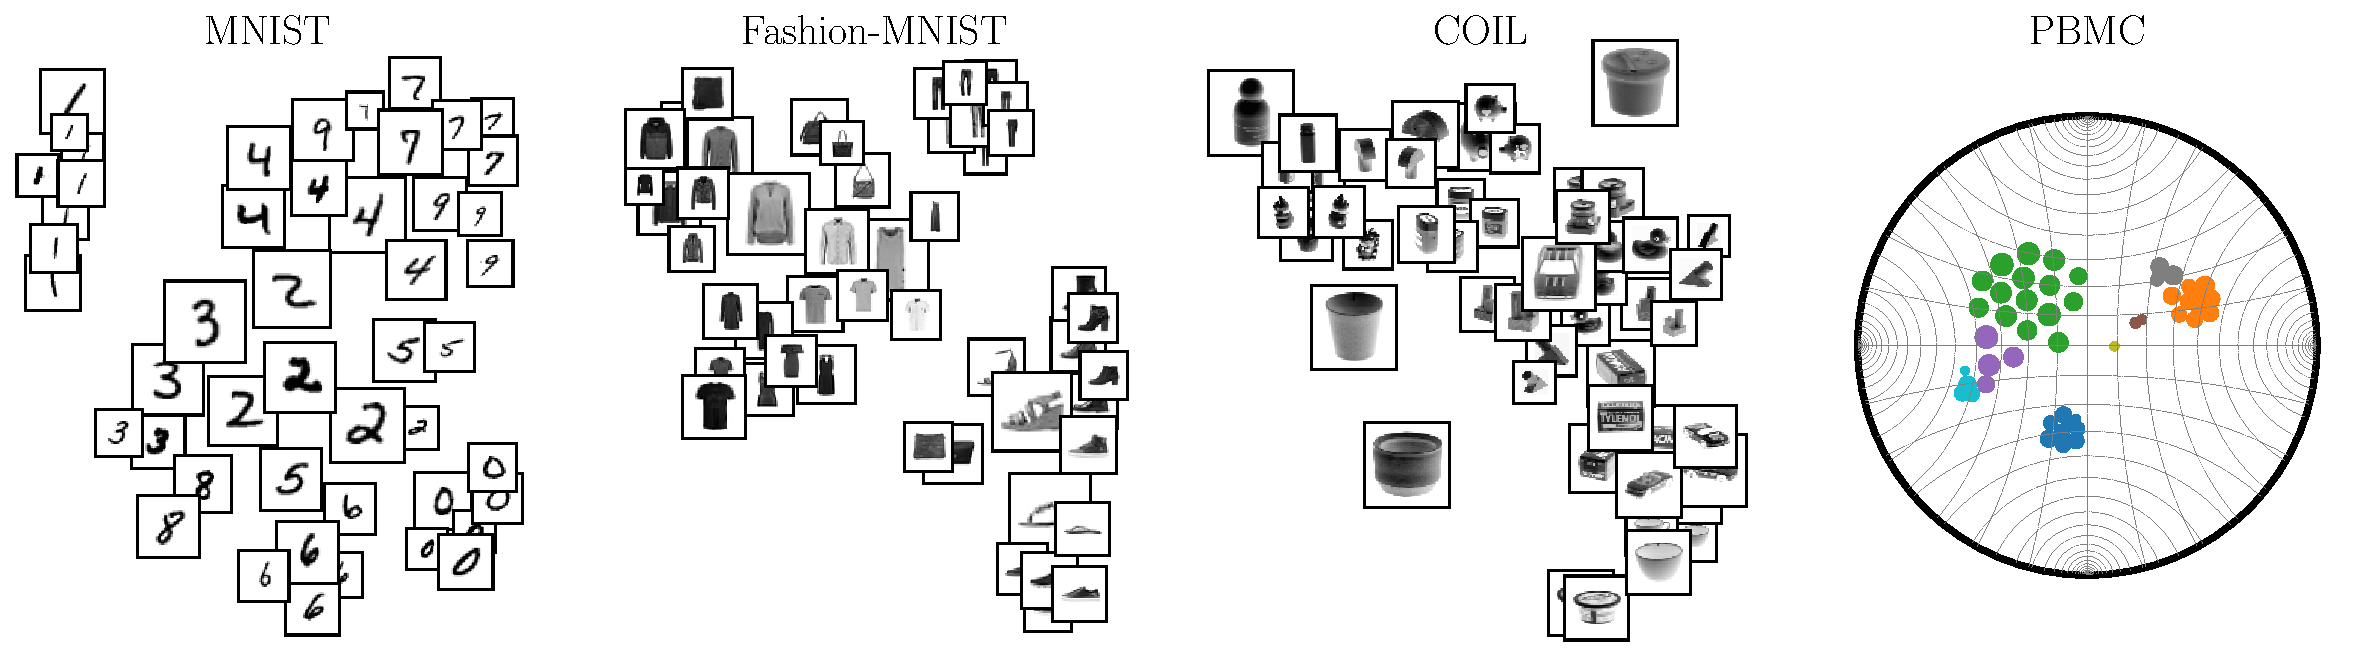
\includegraphics[width=\columnwidth]{figures/DistR/DistDR_embed.pdf}}
		\caption{Examples of 2-dimensional embeddings produced by DistR using the SEA similarity for $\simiX$ 
		and the Student's kernel for $\simiZ$. The latter computed in $\R^2$ for the first three datasets and the Poincaré ball for the last one.
		Displayed images are medoids for each cluster \ie $\argmax_i [\simiX(\mX)\mT_{:,k}]_i$ for cluster $k$. The area of image $k$ is proportional to $[\vh_Z]_k$.
		}
		\label{fig:visu_gwdr}
	\end{center}
	\vspace{-0.8cm}
\end{figure*}


\paragraph{Results.} 
First, we illustrate in \Cref{fig:trade_off} the best trade-off between the aforementioned metrics achieved by all methods.  %across all validated configurations.
For each method and dataset, we considered the model maximizing the sum of the
two normalized metrics to account for their different ranges. DistR, being
present on the top-right of all plots, provides on average the most discriminant
low-dimensional representations endowed with a simple geometry, seconded by
C$\rightarrow$DR. The significant variance of these dynamics for all methods
emphasize the difficulty of performing jointly clustering and DR.
Interestingly, we show in Appendices
\ref{sec:supp_hom_vs_sil}-\ref{sec:supp_hom_vs_nmi} that DistR is the best
suited to describing most datasets at various granularities in low-dimension. %As
For a given configuration, DistR leads to the most consistent performance over
$n$ on average across datasets.\\
% To succinctly illustrate this matter, 
We then display in  \Cref{fig:sensitivity_main} the scores obtained with the neighbor embedding model for several datasets and across all considered number of prototypes $n$. Other kernels and datasets are illustrated in %Figures \ref{fig:sensitivity_sne} and \ref{fig:sensitivity_ip} in the
\Cref{sec:full_sensitivity}. Interestingly, looking at the homogeneity score
(third row), one can notice that DistR is at least as good as C$\to$DR for
grouping points of the same label, even though C$\to$DR performs clustering in
the high dimensional input space. DistR is also generally better than sequential
approaches at representing a meaningful structure of the prototypes in
low-dimension, measured by the silhouette and k-means NMI scores. Therefore, our
approach DistR seems to effectively achieve the best equilibrium between
homogeneity and preservation of the structure of the prototypes. For a
qualitative illustration, we also plot some embeddings produced by our method in
\Cref{fig:visu_gwdr}.

\paragraph{Conclusion.}
By making a connection between the GW problem and popular clustering and DR
algorithms, we proposed a unifying framework denoted as DistR.
DistR enables transforming any DR algorithm into a joint DR-clustering method that produces embeddings (or \emph{prototypes}) with chosen granularity.
We believe that the versatility of the GW framework will enable new extensions in unsupervised learning.
For instance, the formalism associated with (semi-relaxed) GW barycenters naturally enables considering multiple inputs, potentially unaligned and of different sizes. Hence our approach can be useful to address challenges related to the multi-view dimensionality reduction and clustering problems. Other promising directions involve, better capturing multiple dependency scales in the input data by hierarchically adapting the resolution of the embedding similarity graph, or enabling batch optimization of embeddings to operate over much larger datasets.